\section{Nested-Word Automata and Overview of the Library's Organization}
\label{Se:Nested Word Automata}

WALi-NWA is a library for constructing, querying, and operating on
nested-word automata.  It is implemented in C++.  The NWA portions of WALi
are largely logically separate from the rest of WALi, but WALi-NWA does use
facilities provided by WALi and inter-operates with WALi's pushdown system
(PDS) code.

\subsection{Nested Words and Nested-Word Automata}
%\label{Se:Def}

Nested-word automata (NWAs)~\cite{DLT:AM2006,JACM:AM09} are a generalization
of finite-state automata that can capture the matched-parenthesis structure
that is exhibited by, for example, opening and closing tags in XML and the
call/return structure exhibited by execution traces in multi-procedure
programs. Their languages represent somewhat of a middle-ground between
standard regular languages and context-free languages. Nested-word languages
retain the call/return structure mentioned above, which makes them a
refinement of standard regular languages. For instance, there is an NWA that
accepts exactly the language of properly-balanced parentheses (with the
associated matching structure). However, they also retain all the closure
properties that makes standard regular languages attractive; in particular,
they are closed under complementation and intersection. However, they are not
directly comparable to languages of linear words, as the call/return
structure is an explicit part of each word of a nested-word language.

We assume the reader is familiar with the definition of nested words and
nested-word automata; if not, \TODO{appendix A} provides a definition and
Alur et al~\cite{DLT:AM2006,JACM:AM09} describe them in detail. Our
implementation corresponds to the definition from the DLT 2006
paper~\cite{DLT:AM2006}; relative to followup work, this definition removes
the distinction between the machine's linear and hierarchical states, and on
a call always stacks the source state. (In the JACM 2009 presentation of the
work~\cite{JACM:AM09}, this would be called a ``weakly-hierarchical'' NWA.)

Finally, the terminology used in the interface of the package is geared
toward program analysis, so we use terms such as ``call site'' and ``return
site'' to refer to states of the NWA even though they take on different
meanings in different contexts.


\subsection{Library overview}

The core of the NWA library is in the namespace \texttt{wali::nwa}. It
consists of the classes \texttt{NestedWord}, \texttt{NWA},
\texttt{ClientInfo}, and \texttt{WeightGen}.

There are three sub-namespaces that provide functions for operating on NWAs:
\texttt{wali::nwa::query}, \texttt{wali::nwa::construct}, and
\texttt{wali::nwa::nwa\_pds}.

Finally, there are some operations and classes provided by WALi that the NWA
portion of the library uses. This mostly consists of the key-handling code,
but can also include the WPDS portions of the library.

\subsubsection{NWA core classes}

These types live in namespace \texttt{wali::nwa}:

\begin{description}
  \item\texttt{NestedWord} This class models a single nested word. (It can be
    balanced or unbalanced.) To use, include \texttt{wali/nwa/NestedWord.hpp}.
  \item\texttt{NWA} Models nested-word automata themselves. To use, include
    \texttt{wali/nwa/NWA.hpp}, or \texttt{wali/nwa/NWAFwd.hpp} if a
    definition is not needed.
  \item\texttt{NWARefPtr} is a typedef of \texttt{ref\_ptr$<$NWA$>$} (see
    below). This is defined in \texttt{wali/nwa/NWAFwd.hpp}.
  \item\texttt{State} and \texttt{Symbol} are both typedefs of
    \texttt{wali::Key} (see below). Both are defined in
    \texttt{wali/nwa/NWAFwd.hpp}.
  \item\texttt{StateSet} and \texttt{SymbolSet} are typdefs of
    \texttt{std::set}s of the corresponding type. Both are defined in
    \texttt{wali/nwa/NWAFwd.hpp}. (Client code should not depend on this
    fact; it could change to be an \texttt{unordered\_map} or other similar
    container.) These are also defined in \texttt{wali/nwa/NWAFwd.hpp}.
  \item\texttt{ClientInfo} This class holds client-specific information that
    is associated with a state. Client code can subclass ClientInfo and use
    members of the \texttt{NWA} class to attach instances to states. To use,
    include \texttt{wali/nwa/ClientInfo.hpp}.
  \item\texttt{WeightGen} This abstract class describes how to assign weights
    to transitions of the NWA, and is used both when converting an NWA to a
    PDS and when doing prestar/poststar queries on the NWA directly. To use,
    include \texttt{wali/nwa/WeightGen.hpp}.
\end{description}


\subsubsection{NWA free functions}

The library provides a large number of free functions for operating on
NWAs. These are partitioned into the following namespaces (include paths are
relative to the \texttt{Source} directory):

\begin{description}
  \item\texttt{wali::nwa::query} This namespace provides functions for
    querying an automaton. The kinds of functions in this namespace are:
    \begin{itemize}
      \item A large quantity of functions that query transitions of
        the NWA, returning information about one of the states or the symbol
        in transitions that meet some criteria. (For example, ``give me all
        states that appear as the target state of an internal transition with
        this source state.'')
      \item prestar and poststar functions on an NWA
      \item Determining whether two NWAs have any states in common
      \item Determining whether the languages of two NWAs are equal, or if
        one is a subset of the other
      \item Determining whether the language of an NWA is empty
      \item Determining whether a \texttt{NestedWord} is a member of the
        language of an NWA
      \item Determining whether an \texttt{NWA} is deterministic
    \end{itemize}
  \item\texttt{wali::nwa::construct} This namespace provides functions for
    constructing an NWA. Functions in this namespace are standard,
    language-theoretic operations such as intersection, union, concatenation,
    Kleene star, and reversing.
  \item\texttt{wali::nwa::nwa\_pds} This namespace provides functions for
    converting between NWAs and PDSs, and related functions. (Note that
    construction of an NWA from a PDS is in this namespace, not in
    \texttt{construct}.)
\end{description}


\subsubsection{Generic WALi}

The NWA library uses these portions of the standard WALi library. Unless
otherwise specified, they are in namespace \texttt{wali}. See \cite{wali}.

\begin{description}
  \item\texttt{ref\_ptr$<$T$>$} This is a reference-counted intrusive smart
    pointer template.
  \item\texttt{Key} This is a unique identifier for states and symbols in an
    NWA or NestedWord. It is actually a typedef of an integer, though client
    code should not depend on this fact. Note that the use of keys for both
    states and symbols means that they can be confused from a types
    perspective, so use caution that this does not happen. See \cite{wali}.
  \item\texttt{getKey(...)} This function produces a key from some input. If
    the input has not been seen before, it returns a new key; if it has, then
    it returns the same key as before. (One can think of this as translating
    whatever unique identifier is known by the client code to the
    \texttt{Key} needed by WALi.) Versions of this function are provided for
    the following types:
    \begin{itemize}
      \item \texttt{std::string const \&}
      \item \texttt{char *}
      \item \texttt{int}
      \item \texttt{std::set<Key> const \&}
      \item \texttt{key, Key} (this is a two-argument version of
        \texttt{getKey})
      \item \texttt{key\_src\_t}
    \end{itemize}

    The final overload, for \texttt{key\_src\_t}, is a \texttt{ref\_ptr} to a
    \texttt{KeySource} object. \texttt{KeySource} is an abstract class which
    client code can subclass to provide a translation to \texttt{Key}s for
    arbitrary types.
  \item\texttt{key2str} Is a inverse of \texttt{getKey}, except that it
    always returns a string representation. If the key was created with the
    \texttt{getKey(std::string const \&)} overload in the first place, this
    returns a copy of the original string.
  \item\texttt{wali::wfa::WFA} This is a weighted finite automaton. It is
    used in NWA poststar and prestar queries in much the same manner as in
    WPDS poststar and prestar queries.
  \item\texttt{wali::wpds::WPDS} This is a weighted pushdown system. NWAs use
    WPDSs behind the scenes when doing poststar and prestar queries, and the
    library provides conversion routines between the two automata types.
\end{description}


\subsection{Construction}
\label{Se:Construction}

The NWA provides two constructors, the default constructor and the copy
constructor. The default constructor creates an empty NWA. Thereafter, 
client code can \begin{inparaenum} \item add or remove states, \item add or remove
symbols, \item add or remove transitions, \item set the status of certain
  states as initial or final, and \item combine component NWAs (via union,
  intersection, etc). \end{inparaenum}


The following functions are related to construction:
\begin{description}
  \item \texttt{NWA::NWA()}) constructs an empty NWA

  \item \texttt{NWA::NWA(NWA const \& other)} Copies \texttt{other}; the
    automata will not share structure

  \item \texttt{NWA::operator=(NWA const \& other)} Assigns \texttt{other} to \texttt{this};
    the automata will not share structure.

  \item \texttt{NWA::clear()} \nopagebreak
    Removes all states, symbols, and transitions from the NWA.

\end{description}



\subsection{Examples}
\label{Se:Examples}

As an example, consider the nested word automaton $A = (Q_A, \Sigma_A,
{Q_0}_A, \delta_A, F_A)$ where $Q_A = \{Start, Call, Entry, State, Exit,
Return, End\}$, $\Sigma_A = \{a,
call, b, ret\}$, ${Q_0}_A = \{Start\}$, $F_A = \{End\}$, and \\
$\delta_A = 
\begin{cases} 
\delta_i = \{(Start,a,Call), (Entry,b,State), (State,b,Exit), (Return,a,End)\}, \\
\delta_c = \{(Call,call,Entry)\}, \\ 
\delta_r = \{(Exit,Call,ret,Return)\}, \\ 
\end{cases}$ \\
as seen in Figure \ref{Fig:Example1}.
 
\begin{figure}[htb]
  \centering
    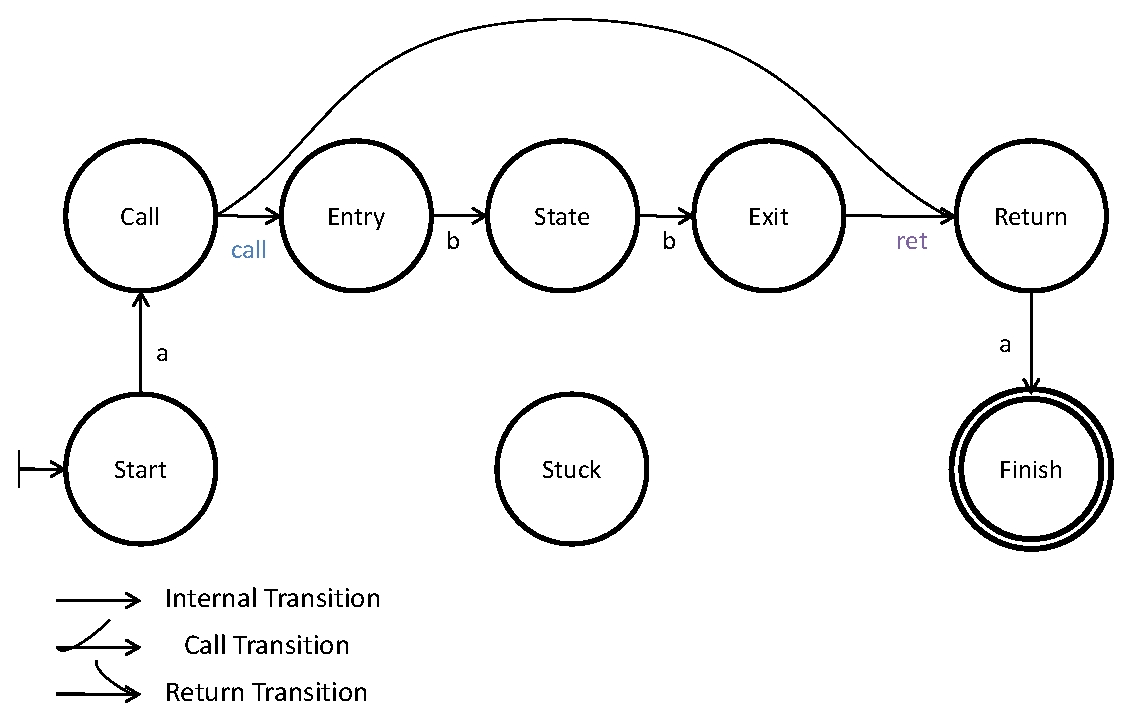
\includegraphics[width=12cm]{Figures/Figure1}
  \caption{An example NWA.}
  \label{Fig:Example1}
\end{figure}

